\documentclass[fr]{../../../eplsummary}

\usepackage[french,ruled,vlined]{algorithm2e}
\usepackage[minted]{../../../eplcode}

\DeclareMathOperator{\dom}{dom}
\DeclareMathOperator{\image}{image}

\newcommand{\halt}{\textnormal{halt}}
\newcommand{\HALT}{\textnormal{HALT}}
\newcommand{\diag}{\textnormal{diag}}
\newcommand{\interpret}{\textnormal{interpret}}

\renewcommand{\epsilon}{\varepsilon}
\renewcommand{\theta}{\vartheta}
\renewcommand{\kappa}{\varkappa}
\renewcommand{\rho}{\varrho} % remember my teacher and friend Adalberto!
\renewcommand{\phi}{\varphi}
\newcommand{\smn}{s_n^m}

\renewcommand{\bar}[1]{\overline{#1}}

\hypertitle{Calculabilité}{6}{INGI}{1123}
{Gilles Peiffer\and Liliya Semerikova}
{Yves Deville}

\section{Introduction}

\subsection{Qu'est-ce que la calculabilité?}
\begin{mydef}
La \emph{calculabilité} étudie les \emph{limites} de l'informatique,
des langages de programmation, des ordinateurs et des systèmes formels,
indépendamment des lois physiques des machines
et des langages et méthodes de programmation existants.
Il existe deux types de limites: théorique et pratique.
Pour la calculabilité,
on s'occupe des limites théoriques alors que
pour la \emph{compléxité} on s'occupe des limites pratiques.
Un problème est dit \emph{calculable} s'il existe un programme
qui résout ce problème.
\end{mydef}
La calculabilité permet donc uniquement de
dire si oui ou non un programme peut être écrit pour résoudre un problème donné.
Lorsqu'un problème est non calculable,
cela nous informe qu'il n'existe pas de programme pour résoudre ce problème.

\begin{mydef}
	En informatique, une \emph{information} est un objet formel,
	un symbole, sans signification propre.
	Le \emph{traitement de l'information} est une manipulation automatique
	d'un objet formel afin de produire un nouvel objet.
	On \emph{spécifie} un programme avec des pré/postconditions
	afin de pouvoir \emph{donner un sens} aux résultats produits.
\end{mydef}

\subsection{Notion de problème}
Il ne faut pas confondre \emph{problème} et \emph{programme}.
Les caractéristiques d'un problème sont:
\begin{itemize}
	\item un problème est \emph{générique}: il s'applique
	à un ensemble de données;
	\item pour chaque donnée particulière, il existe une réponse.
\end{itemize}

On représente un problème par une \emph{fonction}
(noté $\phi$) où la description du problème
est \emph{équivalente} à la description de la fonction.

\subsection{Notion de programme}
Un \emph{programme} est une \og \emph{procédure effective} \fg{},
c'est-à-dire exécutable par une machine.
Étant donné un problème, on souhaite un programme
permettant de résoudre le problème
et on exige qu'un programme soit \emph{correct} et \emph{efficace}.
L'\emph{efficacité} est une \emph{mesure} des ressources
nécessaires à mettre en \oe{}uvre pour que
le programme produise les résultats attendus.
On définit la notion de la \emph{compléxité} indépendamment du formalisme,
de la machine et du contexte technologique utilisé.
C'est cela qui va définir la frontière entre
le \og faisable en pratique \fg{} et l'\og infaisable en pratique \fg{}.
Voici quelques problèmes majeurs
qu'un ordinateur peut accomplir théoriquement,
mais qui, en pratique, ne peuvent pas être résolus:
\begin{itemize}
	\item équivalence des langages de programmation;
	\item problèmes non calculables;
	\item problèmes intrinséquement complexes.
\end{itemize}

\subsection{Résultats pricipaux}
\subsubsection{Équivalence des langages de programmation}
D'un point de vue théorique,
les langages de programmation sont tous \emph{équivalents}.
Un problème est donc calculable indépendamment du langage utilisé,
à condition que le langage soit \emph{complet}.
D'un point de vue pratique,
certains langages sont mieux adaptés que d'autres
pour certaines \emph{classes de problèmes}.

\subsubsection{Existence des problèmes non calculables}
Prenons un exemple de problème non calculable: la détection des virus.

\begin{mydef}
	Un programme est dit \emph{nuisible} si son exécution
	a pour effet de contaminer d'autres programmes.
	Il est considéré comme \emph{dangereux}
	lorsqu'il rend la machine partiellement ou totalement inutilisable.
\end{mydef}

Un bon logiciel antivirus serait alors un programme \texttt{detecteur(P, D)}
qui testerait des programmes en regardant s'ils se multiplient,
tout en les empêchant de modifier d'autres fichiers.
Les spécification du programme \texttt{detecteur(P, D)}:
\begin{itemize}
	\item \emph{Préconditions}: un programme \texttt{P}
	et une donnée \texttt{D}.
	\item \emph{Postconditions}: \og \texttt{"Mauvais"} \fg{}
	si \texttt{P(D)} est nuisible,
	\og \texttt{"Bon"} \fg{} sinon.
\end{itemize}

\begin{mytheo}
	Il n'est pas possible d'écrire un programme antivirus non nuisible
	qui puisse déterminer avec sûreté
	si un programme \texttt{P} est nuisible avec une entrée \texttt{D}.
\end{mytheo}
\begin{proof}
Il faut aussi que le détecteur ne soit pas nuisible
pour que cette spécification soit valide.
Or comme nous allons le démontrer, le détecteur ne peut être non nuisible.
Pour le prouver nous allons émettre l'hypothèse
qu'un programme \texttt{detecteur(P, D)} existe et qu'il n'est pas nuisible.
Dans ce cas, nous pouvons construire le programme \texttt{drole(P)} suivant:

\begin{algorithm}[H]
\DontPrintSemicolon
\KwData{Un programme \texttt{P}.}
\KwResult{Stop si \texttt{detecteur(P, P) = "Mauvais"},
infection d'un autre programme en y insérant \texttt{P} sinon.}
\Begin{
	\eIf{\texttt{detecteur(P, P) = "Mauvais"}}{
		STOP\;
	}{
		Infecter un autre programme en y insérant \texttt{P}\;
	}
}
\caption{\texttt{drole(P)}\label{algo:droleP}}
\end{algorithm}

Regardons maintenant si l'exécution de \texttt{drole(drole)},
c'est-à-dire si l'on donne le code source de \texttt{drole} à lui-même,
est nuisible ou non.
L'algorithme devient alors

\begin{algorithm}[H]
\DontPrintSemicolon
\KwData{Le programme \texttt{drole} lui-même.}
\KwResult{Stop si \texttt{detecteur(drole, drole) = "Mauvais"},
infection d'un autre programme en y insérant \texttt{drole} sinon.}
\Begin{
	\eIf{\texttt{detecteur(drole, drole) = "Mauvais"}}{
		STOP\;
	}{
		Infecter un autre programme en y insérant \texttt{drole}\;
	}
}
\caption{\texttt{drole(drole)}\label{algo:droledrole}}
\end{algorithm}

\begin{itemize}
	\item Supposons que \texttt{drole(drole)} soit nuisible.
	Lorsqu'on exécute, \texttt{detecteur(drole,drole)} n'infecte rien
	car \texttt{detecteur} n'est pas nuisible.
	Comme \texttt{detecteur} retourne \og \texttt{"Mauvais"} \fg{},
	le programme s'arrête.
	Rien n'a donc été infecté, ce qui est contradictoire
	avec le fait que \texttt{drole} soit nuisible.
	\item Si l'exécution de \texttt{drole(drole)} n'est pas nuisible,
	alors \texttt{detecteur(drole, drole)}
	ne va pas retourner \og \texttt{"Mauvais"} \fg{}
	et le code de la clause \texttt{else} s'éxécutera.
	Un autre programme est alors infecté,
	ce qui contredit le fait que \texttt{drole(drole)} ne soit pas nuisible.
\end{itemize}

On a donc une contradiction dans tous les cas,
ce qui implique que le programme \texttt{detecteur} ne peut pas exister.
\end{proof}

\subsubsection{Existence de problèmes intrinsèquement complexes}
\begin{mydef}
	Un \emph{problème intrinsèquement complexe}
	est un problème pour lequel le meilleur algorithme
	n'a pas une complexité polynomiale.
	On dit qu'un algorithme avec une complexité polynomiale
	est efficace car une augmentation multiplicative
	de la puissance des ordinateurs
	se traduit en une augmentation multiplicative aussi
	de la taille maximale des problèmes résolubles.
	Pour une complexité exponentielle,
	la taille maximale résoluble n'augmente que d'un facteur additif.
\end{mydef}

\subsection{Objectifs, calculabilité et complexité}

\begin{figure}[H]
	\centering
	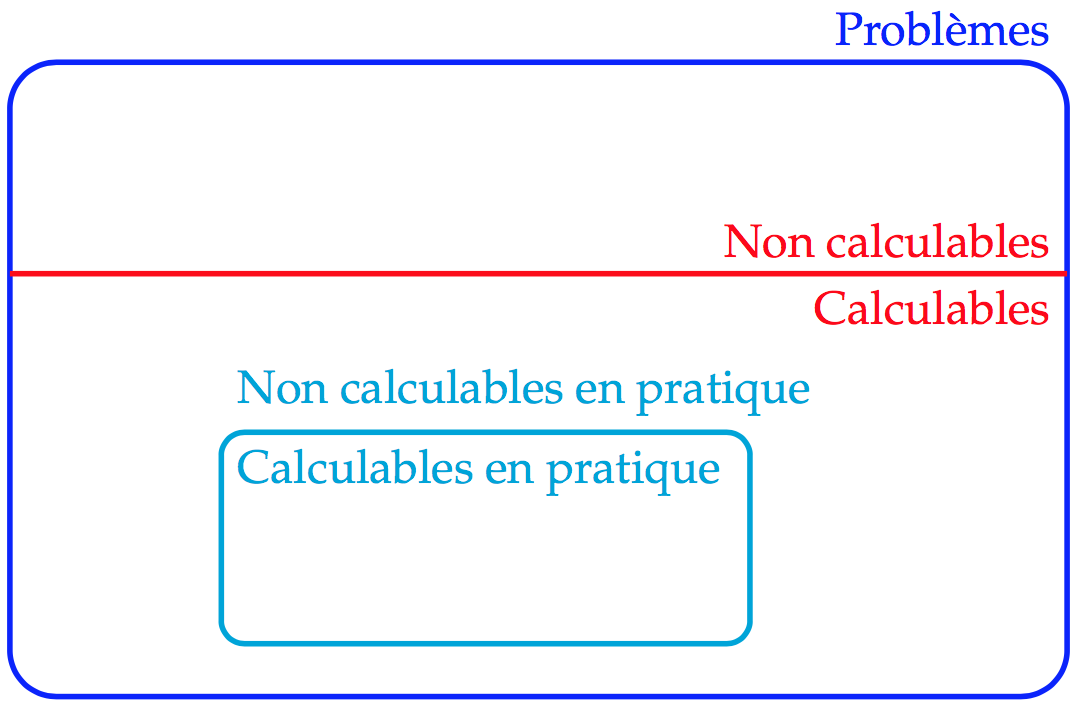
\includegraphics[width=0.5\textwidth]{img/limite_calcu}
	\caption{Problèmes calculables/non calculables.}
\end{figure}

L'intérêt de la calculabilité est de savoir quels problèmes sont calculables
ou lesquels ne le sont pas.
Si un problème est non calculable,
il est inutile d'essayer de résoudre ce problème.
Certains problèmes, quoique théoriquement solubles par un programme,
sont en pratique infaisables, car nécessitant des ressources
incompatibles avec les réalités physiques.
Ce sont les \emph{problèmes intrinséquement complexes}.
En pratique, on utilise souvent des algorithmes efficaces
qui permettent de trouver une solution qui se rapproche de la solution optimale
mais ne fournissent qu'une \emph{approximation}.

\section{Concepts}
\subsection{Ensemble, langages, relations et fonctions}
\subsubsection{Ensembles}
\begin{mynota}
	\begin{description}
		\item[Ensemble vide:] $\emptyset$
		\item[Ensemble fini:] exemple: $\{\,0, 1, 2, \ldots, n\,\}$
		\item[Ensemble infini:] exemple: $\{\,0, 1, 2, \ldots\,\}$
		\item[Produit cartésien:] $A \times B$
		\item[Nombre d'éléments:] $\abs{A}$
		\item[Ensemble des sous-ensembles:] $\mathcal{P}(A)$ ou $2^A$;
		exemple: $2^{\{0, 1\}} = \{\,\emptyset, \{\,0\,\}, \{\,1\,\}, \{\,0, 1\,\}\,\}$.
		On a la propriété $\abs{2^A} = 2^{\abs{A}}$.
		\item[Complément:] $\bar{A}$
	\end{description}
\end{mynota}

\subsubsection{Langages}
\begin{mydef}\leavevmode
\begin{itemize}
	\item Un \emph{ensemble} est une collection d'objets, sans répétition,
	appelés les éléments de l'ensemble.
	\item Une \emph{chaîne de caractères}, ou un \emph{mot},
	est une séquence finie de symboles juxtaposés (éléments de l'alphabet).
	On note $\varepsilon$ la chaîne de caractères vide.
	\item Un \emph{alphabet} $\Sigma$ est un ensemble de symboles.
	L'ensemble des mots possibles sur cet alphabet se note $\Sigma^*$
	\item Un \emph{langage} est un ensemble de mots
	constitués de symboles d'un alphabet donné.
\end{itemize}
\end{mydef}

\subsubsection{Relations}
\begin{mydef}
Soient $A$, $B$ deux ensembles.
Alors une \emph{relation} $R$ sur $A$, $B$ est un sous-ensemble de $A \times B$,
donc un ensemble de paires $\langle a, b \rangle$ avec $a \in A, b \in B$.
Une relation est définie par sa table: $\langle a,b \rangle \in R, aRb, R(a,b)$.

Une \emph{fonction} $f \colon A \to B$ est une relation
telle que pour tout $a \in A$,
il existe au plus un $b \in B$ tel que $\langle a,b \rangle \in f$,
ce qui est équivalent à écrire: $f(a) = b$.
Si $a \in A$ et qu'il n'existe pas de $b \in B$ tel que $f(a) = b$,
alors $f(a)$ est \emph{indéfinie}, noté $f(a) = \bot$.
Le symbole $\bot$ est appelé \emph{bottom}.
\end{mydef}

\paragraph{Propriétés des fonctions}
\begin{myprop}
Soit $f \colon A \to B$
\begin{itemize}
	\item Le \emph{domaine} de $f$ est $\dom f = \{\,a \in A : f(a) \ne \bot\,\}$.
	\item L'\emph{image} de $f$ est $\image f  = \{\,b \in B : \exists a \in A : b = f(a)\,\}$.
	\item La fonction $f$ est une fonction \emph{totale} si $\dom f = A$.
	\item La fonction $f$ est une fonction \emph{partielle}
	si $\dom f \subseteq A$.
	\item La fonction $f$ est \emph{surjective} si $\image f = B$.
	\item La fonction $f$ est \emph{injective} si $\forall a,
	a' \in A : a \ne a' \implies f(a) \neq f(a')$.
	\item La fonction $f$ est \emph{bijective}
	si $f$ est totale, injective et surjective.
\end{itemize}
\end{myprop}

\begin{mydef}
Soient $f, g \colon A \to B$.
\begin{itemize}
	\item La fonction $f$ est une \emph{extension} de $g$
	si $\forall x \in A: g(x) \ne \bot \implies f(x) = g(x)$
	et $f$ a la même valeur que $g$ partout où $g$ est définie.
\end{itemize}
\end{mydef}

Une \emph{fonction} est définie par sa table (peut-être infinie).
On peut définir une fonction
\begin{itemize}
	\item par un \emph{texte fini}
	déterminant sans contradiction ni ambiguïté le contenu de sa table;
	\item par un \emph{algorithme}
	(définissant aussi un moyen de calculer la fonction);
	\item en \emph{énumérant} les paires de la relation.
\end{itemize}
Le fait de savoir définir une fonction précisément
n'implique pas pour autant qu'on connaît un moyen de la calculer.

\subsection{Ensemble énumérable}
\begin{mydef}
	Deux ensembles $A$ et $B$ ont le même \emph{cardinal}
	s'il existe une bijection entre $A$ et $B$.
	Soit $\mathbb{N}$ l'ensemble des nombres naturels.
	Un ensemble est \emph{énumérable}
	ou \emph{dénombrable} s'il est fini
	ou s'il a le même cardinal que $\mathbb{N}$.
	Un ensemble infini est \emph{énumérable}
	s'il existe une liste infinie de tous ses éléments.
\end{mydef}

\subsubsection{Exemples}
On peut montrer que les ensembles suivants sont énumérables:
\begin{itemize}
	\item L'ensemble des nombres naturels, $\mathbb{N}$.
	\item L'ensemble des nombres entiers, $\mathbb{Z}$.
	\item L'ensemble des paires, triples, \ldots, $n$-uplets d'entiers.
	On énumère d'abord les $n$-uplets de somme $0, 1, \ldots$
	\item L'ensemble des rationnels, $\mathbb{Q}$,
	car un rationnel est en fait une paire d'entiers
	en représentation fractionnelle.
	\item L'ensemble des sous-ensembles \emph{finis} d'entiers.
	\item L'ensemble des chaînes finies de caractères sur un alphabet fini.
	\item L'ensemble des fonctions de $\{\,0, 1\,\}$ vers $\mathbb{N}$.
	Attention que l'ensemble des fonctions de $\mathbb{N}$ vers $\{0, 1\}$
	n'est pas énumérable.
	\item L'ensemble des programmes \java.
\end{itemize}

\subsubsection{Propriétés}
\begin{myprop}
Tout sous-ensemble d'un ensemble \emph{énumérable} est \emph{énumérable}.
\end{myprop}
\begin{proof}
	Soit $A$ un sous-ensemble (infini) d'un ensemble $E$ énumérable.
	Comme $E$ est énumérable, il existe une énumération de ses éléments.
	Enlevons de cette liste les éléments qui ne sont pas dans $A$.
	On obtient une nouvelle liste qui énumère les éléments de $A$.
\end{proof}

\begin{myprop}
L'\emph{union} et l'\emph{intersection}
de deux ensembles énumérables sont énumérables.
\end{myprop}
\begin{proof}
	Soient $A$ et $B$ deux ensembles énumérables infinis.
	Leur intersection est énumérable car elle est un sous-ensemble de $A$,
	par la propriété précédente.
	Les éléments des ensembles $A$ et $B$
	peuvent être listés ($A=\{\,a_0, a_1, \ldots ,a_n,\ldots\,\}$
	et $B=\{\,b_0, b_1,\ldots,b_n,\ldots\,\}$).
	Les éléments de $A \cup B$ peuvent être également listés:
	$a_0, b_0, a_1, b_1, \ldots,a_n,b_n,\ldots$
	en y retirant ensuite les doublons.
	Donc, $A \cup B$ est énumérable.
\end{proof}

\begin{myprop}
L'union d'une infinité énumérable d'ensembles énumérables est énumérable.
\end{myprop}
\begin{proof}
	On met chaque ensemble en ligne,
	il y a un nombre énumérable de lignes
	qu'on peut donc numéroter avec des naturels.
	En parcourant le tableau en diagonale montante en partant de $(0,0)$,
	on a un algorithme qui passe sur tous les éléments de l'ensemble.
\end{proof}

\begin{myprop}
	Tout ensemble de chaînes finies de caractères
	sur un alphabet fini est énumérable.
\end{myprop}
\begin{proof}
	C'est un sous-ensemble de l'ensemble
	de toutes les chaînes finies de caractères, qui est énumérable.
\end{proof}

\begin{myprop}
	L'ensemble des programmes \java{} est énumérable.
\end{myprop}
\begin{proof}
Un programme \java{} est une séquence finie d'un alphabet fini.
Il y a donc potentiellement autant d'éléments qu'il y a de naturels,
ni plus ni moins, ce qui nous donne une bijection
entre programmes et $\mathbb{N}$.
\end{proof}

\begin{myprop}
Tout langage (avec un alphabet fini) est énumérable.
\end{myprop}
\begin{proof}
	Un langage est un ensemble de chaînes finies
	de caractères d'un alphabet fini.
	Il est donc énumérable.
\end{proof}

\begin{myprop}
	L'union d'une infinité non énumérable d'ensembles énumérables
	ne peut pas être énumérable.
\end{myprop}
\begin{proof}
	Par contradiction.
	Soit l'union des singletons pour tout réel $x$.
	Ces singletons sont finis, donc énumérables,
	cependant leur union forme l'ensemble des réels, $\R$,
	dont on sait qu'il n'est pas énumérable.
	C'est une contradiction,
	et cela prouve le théorème.
\end{proof}

On peut dire qu'un ensemble est énumérable
s'il existe un algorithme qui affiche tous ses éléments.
Plus intuitivement, tout ensemble
dont les éléments peuvent être représentés de manière finie est énumérable.

Pour démontrer qu'un ensemble est énumérable, on peut
\begin{itemize}
	\item montrer qu'il y a une bijection avec $\mathbb{N}$;
	\item montrer que l'ensemble est fini;
	\item écrire un programme qui énumère l'ensemble;
	\item utiliser une des propriétés données.
\end{itemize}

\subsubsection{Diagonalisation de Cantor}

\begin{mytheo}[Indénombrabilité des réels---Cantor, 1874]
	\label{theo:cantor}
	Soit $E = \{\,x \in \R : 0 < x \le 1\}$.
	$E$ est non énumérable.
\end{mytheo}
\begin{proof}
	Par l'absurde.
	En supposant que $E$ soit énumérable,
	on va montrer qu'un nombre $d'$ n'est pas dans l'énumération
	alors qu'on sait que $d'$ est un nombre réel compris entre $0$ et $1$.

	On suppose donc qu'il existe une énumération des éléments de $E$:
	$x_0, x_1, \ldots, x_k, \ldots$
	On peut représenter un nombre $x_k$ entre $0$ et $1$
	comme étant une suite de chiffres $x_{ki}$:
	$x_k=0.(x_{k0})(x_{k1})\cdots(x_{kk})\cdots$
	Si deux écritures sont possibles, on en choisit une.
	On peut donc construire une table infinie:
	\begin{table}[H]
	\centering
	\begin{tabular}
	{|c||c|c|c|c|c|c|}
	\hline
	 & $1$\ieme{} chiffre & $2$\ieme{} chiffre & $3$\ieme{} chiffre & $\cdots$ & $k+1$\ieme{} chiffre & $\cdots$\\
	\hline
	$x_0$ & $x_{00}$ & $x_{01}$ & $x_{02}$ & $\cdots$ & $x_{0k}$ & $\cdots$\\
	$x_1$ & $x_{10}$ & $x_{11}$ & $x_{12}$ & $\cdots$ & $x_{1k}$ & $\cdots$\\
	$x_2$ & $x_{20}$ & $x_{21}$ & $x_{22}$ & $\cdots$ & $x_{2k}$ & $\cdots$\\
	\vdots & \vdots & \vdots & \vdots & $\ddots$ & \vdots & \vdots\\
	$x_k$ & $x_{k0}$ & $x_{k1}$ & $x_{k2}$ & $\cdots$ & $x_{kk}$ & $\cdots$\\
	\vdots & \vdots & \vdots & \vdots & \vdots & \vdots & $\ddots$\\
	\hline
	\end{tabular}
	\end{table}

	Ensuite, on va sélectionner la diagonale,
	qui est un nombre réel compris entre $0$ et $1$, de la forme
	$d=0.(x_{00})(x_{11})\cdots(x_{kk})\cdots$
	On modifie l'élément $d$
	pour obtenir $d'=0.(x'_{00})(x'_{11})\cdots(x'_{kk})\cdots$,
	où on prend la convention (arbitraire)
	que $x'_{ii}=5$ si $x_{ii} \ne 5$ et $x'_{ii}=6$ si $x_{ii}=5$.
	On a toujours que cet élément $d'$ est un réel
	compris entre $0$ et $1$.
	Le nombre $d'$ est dans l'énumération,
	car $E$ est énumérable (par hypothèse).
	Il existe donc $p$ tel que $x_p = d'$,
	avec $x_p = 0.(x_{p0})(x_{p1})\cdots(x_{pp})\cdots$
	et $d' = 0.(x'_{00})(x'_{11})\cdots(x'_{pp})\cdots$
	Il y a une contradiction car $x'_{pp} \ne x_{pp}$
	par la définition de $x'_{ii}$.
	On a donc $d' \ne x_p$ pour tout $p$, ce qui implique que $d'$
	n'est pas dans l'énumération.
	On peut conclure que $E$ n'est pas énumérable.
	Par extension, les réels, dont $E$ est un sous-ensemble,
	ne sont également pas énumérables.
\end{proof}

\subsubsection{Exemples}
On peut montrer que les ensembles suivants ne sont pas énumérables:
\begin{itemize}
	\item L'ensemble des nombres réels $\R$,
	par le Théorème~\ref{theo:cantor}.
	\item L'ensemble des sous-ensembles de $\mathbb{N}$,
	$\mathcal{P}(\mathbb{N})$.
	On montre que $\mathcal{P}(\mathbb{N})$ est en bijection avec $[0, 1]$.
	\item L'ensemble des chaînes infinies de caractères
	sur un alphabet fini.
	\item L'ensemble des fonctions de $\mathbb{N}$ vers $\{0, 1\}$.
	\item L'ensemble des fonctions de $\mathbb{N}$ dans $\mathbb{N}$.
	On passe par un argument
	similaire à celui du Théorème~\ref{theo:cantor}.
\end{itemize}

On peut dire qu'un ensemble est non énumérable
s'il n'existe pas d'algorithme qui affiche tous ses éléments.
Plus intuitivement, tout ensemble
dont les éléments ne peuvent pas être représentés de manière finie
est non énumérable.
Pour démontrer qu'un ensemble est non énumérable, on peut
\begin{itemize}
	\item montrer qu'il y a une bijection avec $\R$;
	\item utiliser la diagonalisation.
\end{itemize}

\subsubsection{Au-delà de l'énumérable}
Les ensembles non énumérables ci-dessus ont la même taille.
Ils ont la puissance du continu.
Pour aller plus loin,
il suffit de considérer
l'ensemble des fonctions de $\R$ dans $\R$,
ainsi que l'ensemble des sous-ensembles de $\R$ ($2^\R$).
Ces ensembles ne peuvent pas être en bijection avec $\R$.
Pour aller encore plus loin,
on prend l'ensemble des sous-ensemble de l'ensemble défini juste avant
et on obtient alors $2^{2^\mathbb{R}}$.
Pour résumer: $\abs{\emptyset} < \abs{\{\,1,2,3\,\}} < \abs{\mathbb{N}} < \abs{2^{\mathbb{N}}} =
\abs{\R} < \abs{2^{\R}} < \abs{2^{2^\R}} < \abs{2^{2^{2^\R}}} < \cdots$

En informatique, on ne considère que les ensembles énumérables,
comme ce sont ceux dont un programme peut traiter.

\section{Résultats fondamentaux}

\subsection{Algorithmes et effectivité}

\begin{mydef}
Un \emph{algorithme} est une procédure
qui peut être appliquée à n'importe quelle donnée
et qui a pour effet de produire un résultat.
Un algorithme n'est pas une fonction,
mais il calcule une (extension de) fonction.
Les caractèristiques d'un algorithme:
\begin{itemize}
	\item constitué d'un ensemble fini d'instructions;
	\item il existe un \emph{calculateur} qui peut exécuter l'algorithme.
\end{itemize}
Dans cette partie du cours,
un algorithme n'impose pas de limite à la taille des données, des instructions
ni de la mémoire disponible mais son utilisation est finie.
\end{mydef}

\subsection{Fonctions calculables, ensembles récursifs et récursivement énumérables}

\begin{mydef}
Une fonction $f$ est \emph{calculable} s'il existe un algorithme qui,
recevant comme donnée n'importe quels nombres naturels $x_1,\ldots,x_n$,
fournit tôt ou tard comme résultat $f(x)$, si celui-ci existe.
Si l'exécution du programme ne se termine pas, alors $f(x)=\bot$.
Il est bien de remarquer que l'existence d'un algorithme
ne veut pas dire qu'on puisse l'écrire réellement.
Une fonction peut être \emph{totale calculable} ou \emph{partielle calculable}.
\end{mydef}

\begin{mydef}
Soit $ A\subseteq \mathbb{N}$; $A$ est un ensemble \emph{récursif}
s'il existe un algorithme qui,
recevant comme donnée n'importe quel nombre naturel $x$,
fournit tôt ou tard comme résultat $1$ si $x \in A$ et $0$ si $x \notin A$.
L'algorithme décide si $x$ est dans $A$ ou non.

$A$ est un ensemble \emph{récursivement énumérable}
s'il existe un algorithme qui,
recevant comme donnée n'importe quel nombre naturel $x$,
fournit tôt ou tard comme résultat $1$ si $x \in A$ et si $x \notin A$,
l'algorithme fourni un résultat ($\ne 1$) ou ne se termine pas.
Un ensemble $A$ est \emph{co-récursivement énumérable} si son complément
$\bar{A} = \mathbb{N} \setminus A$ est récursivement énumérable.
\end{mydef}

\begin{mydef}
La \emph{fonction caractéristique} $X_A$ de $A$ est
\begin{equation}
	X_A \colon \mathbb{N} \to \{0,1\} \quad \textnormal{telle que} \quad
	X_A(x) = \left \{ \begin{array}{ll}
				1\,, & \textnormal{si}\ x \in A\,, \\
				0\,, & \textnormal{si}\ x \notin A\,. \\
		\end{array}
		\right.
\end{equation}
\end{mydef}

\begin{myprop}
$A$ est un ensemble \emph{récursif}
si et seulement si $X_A$ est une fonction totale calculable.
\end{myprop}

\begin{myprop}
$A$ est un ensemble \emph{récursivement énumérable}
si et seulement si $A = \dom f$,
avec $f$ une fonction totale ou partielle calculable.
\end{myprop}

\begin{myprop}
$A$ est un ensemble \emph{récursivement énumérable}
si et seulement si $A$ est vide,
ou $A = \image f$, avec $f$ une fonction \emph{totale} calculable.
Autrement dit, $f$ est une fonction d'énumération de $A$.
\end{myprop}

\begin{myprop}
Un ensemble est récursif si et seulement s'il est
récursivement énumérable ainsi que corécursivement énumérable.
\end{myprop}

\begin{myprop}
Les propriétés des ensembles récursifs:
\begin{itemize}
	\item $A$ récursif implique $A$ récursivement énumérable;
	\item $A$ récursif implique $\bar{A}$ récursivement énumérable;
	\item $A$ récursif implique $\bar{A}$ récursif;
	\item $A$ récursivement énumérable
	et $\bar{A}$ récursivement énumérable implique $A$ récursif;
	\item $A$ fini implique $A$ récursif;
	\item $\bar{A}$ fini implique $A$ récursif.
\end{itemize}
\end{myprop}

\subsection{Thèse de Church-Turing}
La thèse de Turing est un ensemble de théorèmes et de conjectures.
\begin{itemize}
	\item Aucun modèle de la notion de fonction calculable
	n'est plus puissant que les machines de Turing.
	La version moderne est \og une fonction est \emph{calculable}
	s'il existe un programme d'ordinateur qui calcule cette fonction \fg.
	\item Toute fonction calculable
	est calculable par une machine de Turing.
	\item Toutes les définitions formelles de la calculabilité
	connues à ce jour sont équivalentes.
	\item Toutes les formalisations de la calculabilité
	établies par la suite seront équivalentes aux définitions connues.
\end{itemize}

Seul le troisième énoncé peut être démontré,
les autres sont des thèses ou conjectures.
Comme rien n'est jamais venu infirmer cette thèse,
la thèse est universellement reconnue comme vraie.

\subsection{Programmes et fonctions}
Dans le cours on utilise le langage de programmation \java{} comme modèle.

On note $P$ l'ensemble des programmes \java{}
qui recoivent un ou plusieurs entiers comme données
et qui impriment/retournent un résultat.
$P$ est un ensemble infini dénombrable,
car c'est une chaîne de caractères d'un alphabet fini.
$P$ est recursif, car il existe un programme, le compilateur,
qui détermine si une chaîne de caractères est une programme \java{} ou non.
On peut énumérer les programmes \java{} sans répétition:
$P = P_0, P_1, \ldots, P_k, \ldots$,
où $P_k$ est le programme numéro $k$ dans $P$.
On note $\varphi_k^{(n)} \colon \mathbb{N}^n \to \mathbb{N}$
la fonction calculée par $P_k$.
On remarque que l'inégalité entre les programmes $P_i$ et $P_j$
ne permet pas d'affirmer que $\varphi_i \ne \varphi_j$.
Il existe donc une fonction $f \colon \mathbb{N} \to P$ telle que
\begin{itemize}
	\item $f(k) = P_k$;
	\item $f$ est calculable
	\item $k$ et $P_k$ sont deux représentations distinctes d'un même objet.
\end{itemize}

\subsection{Existence de fonctions non calculables}
Il existe beaucoup de fonctions non calculables,
car la cardinalité de l'ensemble des fonctions
de $\mathbb{N}$ dans $\mathbb{N}$ est égale à celle de l'ensemble des réels.
Or, la cardinalité de l'ensemble des programmes \java, $P$,
est égale à celle de l'ensemble des naturels.
Il y a donc une infinité de fonctions non calculables.

\subsection{Problème de l'arrêt}
Soit la fonction $\halt \colon P \times \mathbb{N} \to \mathbb{N}$
telle que $\halt(n, x)=1$ si l'exécution du programme $P_n(x)$
se termine ($\varphi_n (x) \ne \bot$) et $0$ sinon.
La fonction $\halt$ est totale, bien définie et a une table infinie
qui est décrite de manière finie.
\begin{proof}
Supposons $\halt$ calculable.
On peut donc construire une table infinie définissant la fonction $\halt$:
\[
\begin{array}{|c|cccccc|}
\hline
 & 0 & 1 & 2 & \dots & k & \dots\\
\hline
P_0 & \halt(0,0) & \halt(0,1) & \halt(0,2) & \cdots & \halt(0,k) & \cdots \\
P_1 & \halt(1,0) & \halt(1,1) & \halt(1,2) & \cdots & \halt(1,k) & \cdots \\
P_2 & \halt(2,0) & \halt(2,1) & \halt(2,2) & \cdots & \halt(2,k) & \cdots \\
\vdots & \vdots & \vdots & \vdots & \ddots & \vdots & \vdots \\
P_k & \halt(k,0) & \halt(k,1) & \halt(k,2) & \cdots & \halt(k,k) & \cdots \\
\vdots & \vdots & \vdots & \vdots & \vdots & \vdots & \ddots\\
\hline
\end{array}
\]

On va construire la diagonale $\diag(n) = \halt(n,n)$, qui est donc calculable.
Modifions cette diagonale de façon à ce qu'elle reste calculable:
\[
\diag'(n) = \left\{ \begin{array}{l@{\quad}l}
1\,, & \textnormal{si} \ \halt(n,n) = 0\,, \\
\bot\,, & \textnormal{si} \ \halt(n,n) = 1\,.
\end{array} \right.
\]
Donc, $\diag' = P_d$ pour un certain $d$.
Trouvons la valeur de $\diag'(d)$.
\[
\diag'(d) = \left\{ \begin{array}{l@{\quad}l}
1\,, & \textnormal{si} \ \halt(d,d) = 0\,, \\
\bot\,, & \textnormal{si} \ \halt(d,d) = 1\,.
\end{array} \right.
\]

On regarde ensuite les deux cas de figure possibles:
\begin{itemize}
	\item Si $\diag'(d) = 1$,
	alors $\halt(d, d) = 0$.
	Ceci implique que $P_d(d)$ ne se termine pas.
	Or, si $P_d(d)$ ne se termine pas,
	alors $\diag'(d)$ ne se termine pas non plus et $\diag'(d) = \bot$.
	C'est en contradiction avec l'hypothèse.
	\item Si $\diag'(d) = \bot$,
	alors $\halt(d, d) = 1$.
	Ceci implique que $P_d(d)$ se termine.
	Or, si $P_d(d)$ se termine,
	alors $\diag'(d)$ se termine également et $\diag'(d) = 1$.
	C'est de nouveau en contradiction avec l'hypothèse.
\end{itemize}

Donc aucun algorithme ne permet de déterminer
pour tout programme $P_n$ et donnée $x$ si $P_n(x)$ se termine ou non.
La seule possibilité serait d'avoir un langage de programmation
dans lequel tous les programmes se terminent.
La fonction $\halt$ est alors calculable pour les programmes de ce formalisme.
$\halt$ non calculable ne signifie pas que pour un programme $k$ donné,
$\halt(k,x)$ est non calculable.
\end{proof}

On peut alors définir $\HALT$ comme l'ensemble des programmes $k$
et des valeurs $x$ tel que le programme $k$ se termine avec l'entrée $x$.
\[
\HALT = \{\,(n, x) : P_n(x) \ \textnormal{se termine}\,\} \equiv \{\,(n, x) : \halt(n, x) = 1\,\}\,.
\]
Il existe donc un ensemble non récursif $K$ défini comme
\[
K = \{\,n : P_n(n) \ \textnormal{se termine}\,\} \equiv \{\,n : (n, n) \in \HALT\,\} \equiv \{\,n : \halt(n, n) = 1\,\} \equiv \{\,n : \diag(n) = 1\,\}\,.
\]
Il s'agit de l'ensemble des programmes $P_n$ qui se terminent
en recevant comme entrée leur numéro de programme.

\begin{myprop}
Les propriété des ensembles $\HALT$ et $K$ sont:
\begin{itemize}
	\item $K$ et $\HALT$ ne sont pas récursifs;
	\item $K$ et $\HALT$ sont récursivement énumérables;
	\item $\overline{\HALT}$ n'est pas récursivement énumérable;
	\item $\bar{K}$ n'est pas récursivement énumérable.
\end{itemize}
\end{myprop}
\begin{figure}[H]
	\centering
	\begin{subfigure}[t]{0.45\textwidth}
		\centering
		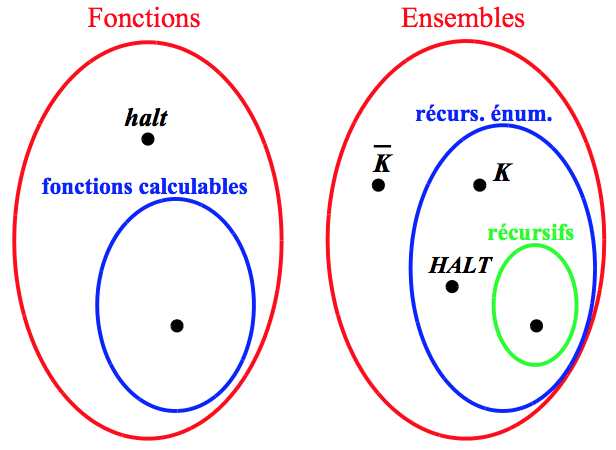
\includegraphics[width=\linewidth]{img/haltk}
		\caption{Comparaison entre
		les structures des fonctions et des ensembles.}
		\label{fig:haltk}
	\end{subfigure}\hfill
	\begin{subfigure}[t]{0.45\textwidth}
		\centering
		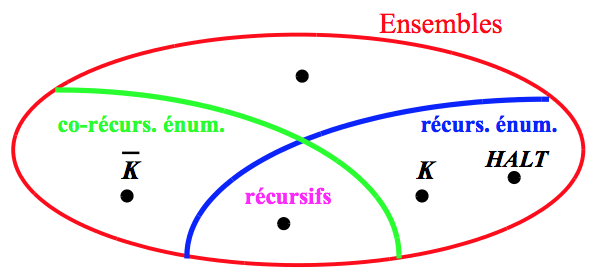
\includegraphics[width=\linewidth]{img/recurs}
		\caption{Vue d'ensemble\footnote{\emph{Pun intended.}}
		des relations entre ensembles
		(co-)récursivement énumérables et récursifs.}
		\label{fig:recurs}
	\end{subfigure}
	\caption{Diagrammes de Venn.}
	\label{fig:venn}
\end{figure}

\subsection{Insuffisance des fonctions totales}
\begin{mytheo}[Théorème de Hoare-Allison]
\label{theo:ha}
Soit un langage de programmation non trivial
et $Q$ l'ensemble des programmes de ce langage tel que
\begin{itemize}
	\item $Q = \{\,Q_0, Q_1, Q_2,\ldots,Q_k,\ldots\,\}$
	et $\varphi'_k$ dénote la fonction calculée par $Q_k$.
	\item Tous les programmes de $Q$ se terminent toujours.
	\item $Q$ possède un interpréteur calculable.
	\item $\interpret(n, x) = \varphi'_n(x)$
	est le résultat de l'exécution du programme $Q_n$ sur la données $x$.
\end{itemize}
Ce langage ne permet pas de calculer toutes les fonctions totales calculables,
car $\interpret(n, x)$ n'est pas calculable dans $Q$.
\end{mytheo}
\begin{proof}
Par diagonalisation de Cantor.
Supposons que \(\interpret\) soit calculable dans \(Q\).
\begin{itemize}
	\item On commence par construire une table
	\[
	\begin{array}{|c|cccccc|}
	\hline
	 & 0 & 1 & 2 & \dots & k & \dots\\
	\hline
	Q_0 & \interpret(0,0) & \interpret(0,1) & \interpret(0,2) & \cdots & \interpret(0,k) & \cdots \\
	Q_1 & \interpret(1,0) & \interpret(1,1) & \interpret(1,2) & \cdots & \interpret(1,k) & \cdots \\
	Q_2 & \interpret(2,0) & \interpret(2,1) & \interpret(2,2) & \cdots & \interpret(2,k) & \cdots \\
	\vdots & \vdots & \vdots & \vdots & \ddots & \vdots & \vdots \\
	Q_k & \interpret(k,0) & \interpret(k,1) & \interpret(k,2) & \cdots & \interpret(k,k) & \cdots \\
	\vdots & \vdots & \vdots & \vdots & \vdots & \vdots & \ddots\\
	\hline
	\end{array}
	\]
	\item On seléctionne la diagonale, $\diag(n) = \interpret(n, n)$.
	\item On modifie \(\diag\) de sorte à ce que
	$\diag' = \interpret(n, n) + 1$ et $\diag'$ soit calculable dans $Q$.
	\item On peut alors dire que $\diag' = Q_d$ pour un certain $d$.
	Par définition de $\diag'$, on a $\diag'(d) = \interpret(d, d) + 1$.
	Or, comme $Q_d$ calcule $\diag'$,
	nous avons aussi $\diag'(d) = \varphi'_d(d) = \interpret(d,d)$.
	Cela mène à une contradiction quant à la valeur de \(\diag'(d)\).
	\item On conclut donc que \(\interpret\) n'est pas calculable dans $Q$.
\end{itemize}
\end{proof}

\begin{myrem}
Si le programmes de $Q$ calculaient également des fonctions partielles,
alors ça n'aurait pas posé de problème, car si $\interpret(d, d) = \bot$,
$\interpret(d, d) + 1 = \bot$ et il n'y a plus de contradiction.
\end{myrem}

\begin{myprop}[Propriétés résultant du Théorème de Hoare-Allison]\leavevmode
\begin{itemize}
	\item Si un language de programmation non trivial
	ne permet que le calcul de fonctions totales, alors:
	\begin{itemize}
		\item l'interpréteur de ce langage
		n'est pas programmable dans ce langage;
		\item il existe des fonctions totales
		non programmables dans ce langage.
	\end{itemize}
	Ce langage est \emph{restrictif}.
	\item Si un langage de programmation non trivial
	permet de programmer son propre interpréteur,
	alors ce langage ne permet pas
	la programmation de la fonction \(\halt\)
	car celle-ci n'est pas calculable.
	\item Il est impossible que l'interpréteur et la fonction \emph{halt}
	puissent être programmés simultanément dans un langage non trivial.
	\item Si on veut qu'un langage de programmation
	permette la programmation de toutes les fonctions calculables,
	alors ce langage doit également permettre
	la programmation de fonctions non totales.
	\item L'ensemble $\{\,n: \varphi_n \textnormal{ est totale}\,\}$
	n'est pas récursif.
\end{itemize}
\end{myprop}

\begin{mytheo}[Existence d'une fonction universelle]
	Il existe \(z\) tel que pour tout \(n, x\),
	\(\phi_z(n, x) = \phi_n(x)\),
	où \(\phi_z\) est une fonction universelle, calculable,
	et \(P_z\) est un programme universel (un interpréteur).
	On note la fonction universelle par \(\theta(n, x) = \phi_z(n, x)\).
\end{mytheo}

\subsection{Extension de fonctions partielles}
\begin{mytheo}[Existence d'une fonction partielle inextensible]
Il existe une fonction partielle calculable $g$
telle qu'aucune fonction totale calculable ne soit une extension de $g$.
\end{mytheo}
\begin{proof}
Par l'absurde.
Définissons une fonction \(g(n, x)\),
qui calcule le nombre d'instructions exécutées par \(\phi_n(x)\).
Cette fonction vaut $\bot$ si $\phi_n(x) = \bot$;
il s'agit donc d'un fonction partielle calculable.
Soit $g'(n,x)$ une extension totale calculable de $g$.
Pour calculer $\halt(n,x)$,
il suffit d'exécuter $g'(n,x)$ instructions de $P_n(x)$.
Si à cette étape, $P_n(x)$ s'arrête, c'est que $g'(n,x) = g(n,x)$
et que $P_n(x)$ se termine.
Si $P_n(x)$ ne s'arrête pas à cette étape,
c'est que $g(n,x) = \bot$ et donc $P_n(x)$ se termine.
On a donc un algorithme pour calculer \(\halt\), ce qui est impossible.
Par déduction, une telle extension totale de $g$ n'existe pas.
\end{proof}

\subsection{Théorème de Rice}
\begin{mydef}[Propriété d'un programme]
	On appelle \emph{propriété d'un programme}
	un sous-ensemble des programmes.
	Ceux qui sont dans le sous-ensemble satisfont la propriété,
	les autres non.
	Une propriété est dite \emph{triviale}
	si le sous-ensemble est vide ou l'ensemble de tous les programmes.
\end{mydef}
\begin{mytheo}[Théorème de Rice, 1951]
\label{theo:rice}
Soit $A \subseteq \N$.
Si $A$ est récursif et $A \neq \emptyset$ et $A \neq \N$,
alors $\exists i \in A$ et $\exists j \in \overline{A}$
tels que $\varphi_i = \varphi_j$.

\begin{figure}[H]
	\centering
	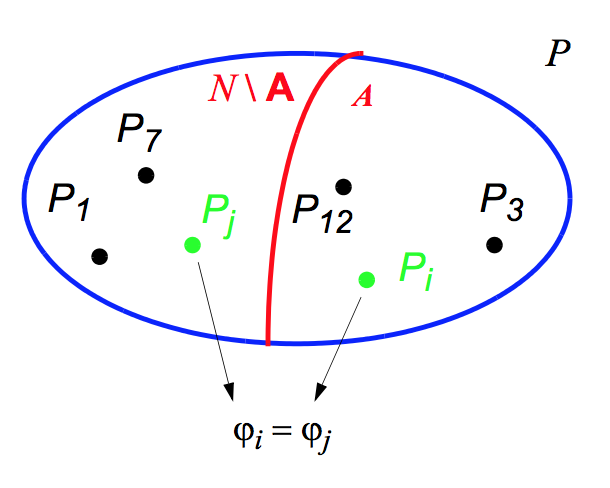
\includegraphics[width=0.7\textwidth]{img/rice}
	\caption{Visualisation du Théorème de Rice.}
\end{figure}

Ceci est équivalent à la contraposée:
si $\forall i \in A$ et $\forall j \in \overline{A}$,
$\varphi_i \ne \varphi_j$,
alors soit $A$ est non récursif, soit $A = \emptyset$ ou $A=\N$.
\end{mytheo}
Informellement, le Théorème~\ref{theo:rice} dit
qu'il est impossible de décider
toute propriété sémantique non triviale d'un programme
à l'aide d'un algorithme.
\begin{proof}
On prouve la contraposée, par réduction.
On suppose donc avoir $\forall i \in A$ et $\forall j \in \overline{A}$,
$\varphi_i \ne \varphi_j$.
Supposons que \(A\) soit récursif et non trivial.

Commençons par construire le programme suivant $P_k$:
\begin{minted}{java}
public static void P_k() {
	while (true) {}
}
\end{minted}
$P_k$ ne s’arrête jamais: $\forall x \varphi_k(x) = \bot$/
On sait par hypothèse que $\overline{A} \ne \emptyset$ car $A \ne \N$.
Supposons s.p.d.g. que $k \in \overline{A}$.
On sait aussi que $A \ne \emptyset$ par hypothèse.
Prenons un élément quelconque $m \in A$.
Par hypothèse, $\forall i \in A$, $\forall j \in \overline{A}$,
$\varphi_i \ne \varphi_j$.
On conclut donc $\varphi_m \ne \varphi_k$.

Pour $n$ et $x$ fixé, analysons le programme \(P_d(z)\) suivant:
\begin{minted}{java}
public static void P_d(int z) {
	P_n(x);
	P_m(z);
}
\end{minted}
La fonction $\varphi_d(z)$ calculée par $P(z)$ se définit comme suit:
\begin{itemize}
	\item Si $P_n(x)$ ne se termine pas,
	alors le programme $P_d(z)$ ne se termine pour aucune valeur de $z$.
	On a donc $\varphi_d = \varphi_k = \bot$.
	\item Si $P_n(x)$ se termine,
	alors le programme $P_d(z)$ calcule le même fonction que $P_m(z)$.
	On a donc $\varphi_d = \varphi_m$.
\end{itemize}
Pour déterminer si $\varphi_d = \varphi_k$
ou $\varphi_d = \varphi_m$, il suffit de tester si $d \in A$.
Par hypothèse, $\forall i \in A$, $\forall j \in \overline{A}$,
$\varphi_i \ne \varphi_j$.
Nous avons aussi $k \in \overline{A} $ et $m \in A$.
\begin{itemize}
	\item Si $d \in A$, alors $\varphi_d \ne \varphi_k$,
	donc $\varphi_d = \varphi_m$.
	\item Si $d \in \bar{A}$, alors $\varphi_d \ne \varphi_m$,
	donc $\varphi_d = \varphi_k$.
\end{itemize}

On résume comme ceci: si $d \in A$,
alors l'exécution de $P_n(x)$ se termine,
sinon l'exécution de $P_n(x)$ ne se termine pas.
On peut alors écrire le programme suivant qui décide \(\HALT\):
\begin{minted}{java}
public static void halt(int n, int x) {
	if A.contains(d) {
		System.out.println(1);
	} else {
		System.out.println(0);
	}
}
\end{minted}
Ceci donne lieu à une contradiction, car \(\HALT\) n'est pas récursif;
l'hypothèse que \(A\) soit récursif est donc fausse.
\end{proof}

\begin{myprop}\leavevmode
\begin{itemize}
	\item Si une certaine propriété est vérifiée par certains programmes,
	mais pas tous, et qu’elle est décidable,
	alors il existe deux programmes calculant la même fonction,
	l’un vérifiant la propriété, l’autre non.
	\item Si la propriété est vérifiée par un programme, mais pas tous,
	alors cette propriété ne peut être décidée par un algorithme.
	\item S’il existe un algorithme permettant de déterminer
	si un programme quelconque
	calcule une fonction ayant cette propriété,
	alors toutes les fonctions calculables ont cette propriété
	ou aucune fonction calculable n’a cette propriété.
	\item Aucune question relative aux programmes,
	vue sous l’angle de la fonction qu’ils calculent,
	ne peut être décidée par l’application d’un algorithme.
	\item Les propriétés intéressantes d’un programme
	concernent la fonction qu’il calcule (sémantique),
	non pas sa forme (syntaxe).
	La plupart des problèmes intéressants au sujet des programmes
	sont donc non calculables.
\end{itemize}
\end{myprop}

\subsection{Théorème de la paramétrisation}
\begin{mydef}[Transformateur de programmes]
	Une fonction $f \colon \N \to \N$ peut être vue
	comme une fonction qui prend le numéro d'un programme et
	qui retourne le numéro d'un autre programme,
	c'est-à-dire $f\colon P \to P$.
	Si $P_k$ calcule la fonction $f$ alors $P_k$ peut être vu
	comme un \emph{transformateur de programmes}.
\end{mydef}

\begin{mytheo}[Théorème \(s_{mn}\)---Kleene, 1952]
\label{theo:smn}
Pour tout $m, n \ge 0$,
il existe $\smn \colon \N^{m+1} \to \N$ total calculable tel que pour tout $k$,
$\phi_{k}^{(n+m)}(x_1,\ldots, x_n, x_{n+1}, \ldots, x_{n+m})
= \phi_{\smn(k, x_{n+1}, \ldots, x_{n+m})}^{(n)} (x_1, \ldots,x_n)$.
C'est-à-dire, étant donné $m,n \ge 0$,
il existe un transformateur de programme $\smn$ qui,
recevant comme données un programme $P_k$
à $m+n$ arguments et $m$ valeurs $v_1,\ldots,v_m$,
fournit comme résultat un programme $P$ à $n$ arguments
tel que la fonction calculée par $P(x_1,\ldots,x_n)$ soit la même
que la fonction calculée par $P_k(x_1,\ldots,x_n,v_1,\ldots,v_m)$.
\end{mytheo}
\begin{proof}
Pour prouver que $\smn$ est totale calculable,
on va montrer comment construire un programme
qui calcule $\smn(k,x_{n+1},\ldots,x_{n+m})$.
Tout d'abord, comme $\phi_k$ est calculable,
il existe un programme $P_k(x_1,\ldots,x_{n+m})$.
Il est donc possible de construire un programme \(Q(x_1, \ldots, x_n)\)
qui calcule $P_k(x_1,\ldots,x_{n+m})$.
$x_1,\ldots,x_n$ restent des arguments du programme,
tandis que $x_{n+1},\ldots,x_{n+m}$ deviennent des valeurs fixées.
Le programme qui calcule $\smn(k,x_{n+1},\ldots,x_{n+m})$
n'a plus qu'à retourner le numéro du programme $Q$.
\end{proof}

Le transformateur de programme $\smn$ particularise un programme
à $n+m$ arguments en rendant constants
les $m$ derniers arguments du programme.
$\smn$ est calculable en toute généralité (en fonction de $m$ et de $n$),
indépendamment des programmes à transformer.
Le transformateur $\smn$ est applicable à tous les programmes
à $m+n$ arguments dont on veut particulariser,
d'une quelconque manière, \(m\) arguments.

\subsection{Théorème du point fixe}
\begin{mytheo}[Théorème du point fixe---Kleene, 1952]
\label{theo:fixedpoint}
Soit $n \ge 0$ et $f$ une fonction totale calculable.
Il existe alors $k$ tel que $\phi_k^{(n)} = \phi_{f(k)}^{(n)}$.
C'est-à-dire que, pour tout transformateur de programme $T$,
il existe deux programmes $P_k$ et $P_j$ tels que
\begin{itemize}
	\item $P_j$ soit la transformation de $P_k$ via $T$;
	\item $P_k$ et $P_j$ calculent la même fonction.
\end{itemize}
\end{mytheo}
\begin{proof}
	On commence par définir une fonction
	\begin{equation}
		h(u, v) =
		\begin{cases}
			\phi_{\phi_u(u)}(v) & \textnormal{si } \phi_u(u) \ne \bot\,,\\
			\bot & \textnormal{sinon.}
		\end{cases}
		\label{eq:hdef}
	\end{equation}
	Cette fonction est calculable.

	Ensuite, on utilise le Théorème~\ref{theo:smn} pour \(m = n = 1\),
	et on trouve qu'il existe un transformateur \(s\)
	tel que \(h(u, v) = \phi_{s(u)}(v)\).

	On peut alors définir \(g(u) = f(s(u))\).
	Comme \(f\) et \(s\) sont calculables, \(g\) l'est aussi.
	On peut donc écrire qu'il existe \(k'\)
	tel que \(\phi_{k'}(u) = g(u) = f(s(u))\).
	Ici, \(k'\) est une constante,
	et \(h(k', v) = \phi_{s(k')}(v)\).

	Par \eqref{eq:hdef} et parce que
	\(g = \phi_{k'}\) est totale calculable,
	on a \(h(k', v) = \phi_{\phi_{k'}(k')}(v)\).
	Par la définition de \(g\), \(g(u) = \phi_{k'}(u) = f(s(u))\),
	et donc \(h(k', v) = \phi_{f(s(k'))}(v)\).
	En utilisant le résultat obtenu
	en appliquant le Théorème~\ref{theo:smn} plus haut,
	on écrit alors \(\phi_{s(k')}(v) = \phi_{f(s(k'))}(v)\).
	On pose alors \(s(k') = k\), et on ré-écrit:
	\(\phi_k(v) = \phi_{f(k)}(v)\),
	ce qui termine la preuve.
\end{proof}

\subsubsection{Preuve du Théorème de Rice grâce au Théorème du point fixe}
\begin{proof}
Soit un ensemble $A$ tel que
$A \ne \emptyset$ et $\overline{A} \ne \emptyset$.
Il suffit de montrer que si
\begin{equation}
\forall i \in A\,, \forall j \in \overline{A}\,, \varphi_i \ne \varphi_j\,,
\label{eq:ricestatement}
\end{equation}
alors $A$ est non récursif.

En supposant $A$ récursif,
on arrive à une contradiction.
En effet, soient $n \in A$ et $m \in \overline{A}$.
Définissons la fonction
$f(x) = \begin{cases}
		m\,, & \textnormal{si } x \in A\,,\\
		n\,, & \textnormal{si } x \in \overline{A}\,.\\
	\end{cases}$
Comme $A$ est récursif, la fonction $f$ est totale calculable.
Dès lors, par le Théorème~\ref{theo:fixedpoint},
il existe $k$ tel que $\varphi_{f(k)} = \varphi_k$.
\begin{itemize}
	\item Si $k \in A$, alors $f(k) = m$.
	On a donc $\varphi_m = \varphi_k$,
	ce qui est contradiction avec \eqref{eq:ricestatement}
	car $m \in \overline{A}$.
	\item Si $k \in \overline{A}$, alors $f(k) = n$.
	On a donc $\varphi_n = \varphi_k$,
	ce qui est contradiction avec \eqref{eq:ricestatement} car $n\in A$.
\end{itemize}
\end{proof}

\begin{mytheo}[Non-récursivité de \(K\)]
	L'ensemble \(K = \{\,k : P_k(k) \ \textnormal{se termine}\,\}\)
	est non récursif.
\end{mytheo}
\begin{proof}
Soit $P_n$ un programme qui ne s’arrête jamais,
et $P_m$ un programme qui calcule la fonction identité:
\begin{itemize}
	\item $\forall x \varphi_n(x) = \bot$;
	\item $\forall x \varphi_m(x) = x$.
\end{itemize}
Définissons maintenant la fonction suivante:
$f(x) = \begin{cases}
		n\,, & \textnormal{si } x \in K\,,\\
		m\,, & \textnormal{si } x \notin K\,.\\
	\end{cases}$
On montre que par construction, pour tout $k$, $\varphi_{f(k)} \ne \varphi_k$.
\begin{itemize}
	\item Si $k \in K$, alors $\varphi_k(k) \ne \bot$.
	On a donc $f(k) = n$ et $\varphi_{f(k)}(k) = \varphi_n(k)
	= \bot \ne \varphi_k(k)$.
	donc $\varphi_{f(k)} \ne \varphi_k$;
	\item Si $k \notin K$,
	alors $\varphi_k(k) = \bot$,
	$f(k) = m$ et $\varphi_{f(k)}(k)
	= \varphi_m(k) \ne \bot = \varphi_k(k)$
	donc $\varphi_{f(k)} \ne \varphi_k$.
\end{itemize}
Si $K$ est récursif, alors $f$ est totale calculable.
Par le théorème du point fixe,
il devrait donc exister $k$ tel que $\varphi_k \ne \varphi_{f(k)}$.
Or, ceci n'ext pas le cas.
$K$ n’est donc pas récursif.
\end{proof}

\subsection{Autres problèmes non calculables}
\subsubsection{Problème de correspondance de Post}
\begin{myprob}[Problème de correspondance de Post]
Soient deux listes \(U\) et \(V\) de \(k\) mots non vides
sur un alphabet \(\Sigma\):
\begin{itemize}
	\item \(\{\,U = u_1, \ldots, u_k\,\}\);
	\item \(\{\,V = v_1, \ldots, v_k\,\}\).
\end{itemize}
Existe-t-il une suite d'entiers \(i_1, \ldots, i_n\)
telle que les mots \(u_{i_1}, \ldots, u_{i_n}\) et \(v_{1_n}, \ldots, v_{i_n}\)
soient indentiques?
\end{myprob}
Il n'existe pas d'algorithme qui puisse répondre à cette question,
étant donné \(U\) et \(V\).

\subsubsection{Équations diophantines}
\begin{mydef}[Équation diophantine]
	Une \emph{équation diophantine} est une équation polynomiale
	de la forme \(D(x_1, \ldots, x_n) = 0\),
	où \(D\) est un polynôme à coefficients entiers.
\end{mydef}
\begin{myprob}[Équation diophantine]
	Déterminer si une équation diophantine donnée
	possède une solution entière.
\end{myprob}
En 1970, Matiyasevich a prouvé
qu'il n'existe pas d'algorithme
qui puisse résoudre ce problème pour tout équation diophantine.

\subsection{Codage et représentation}
Afin de généraliser la calculabilité aux autres types
que les naturels en représentation décimale,
on peut définir un codage.
\begin{mydef}[Codage]
	Un \emph{codage} est une bijection entre
	le nouveau type et les naturels,
	où chaque objet peut être représenté par un naturel (distinct).
\end{mydef}

Les propriétés d'un codage \(c \colon T \to \N\) sont
\begin{itemize}
	\item la fonction \(c\) est bijective;
	\item les fonctions \(c\) et \(c^{-1}\) sont calculables.
\end{itemize}

\subsection{Nombres calculables}
\begin{mydef}[Nombre réel]
	Tout \emph{nombre réel} est défini comme
	la limite d'une suite (convergente) de nombres rationnels.
	Pour tout \(x \in \R\), il existe une fonction totale
	\(s \colon \N \to \Q\) telle que
	\(\lim_{n \to +\infty} \abs{x - s(n)} = 0\).
\end{mydef}
\begin{mydef}[Nombre calculable]
	Un nombre réel \(x\) est \emph{calculable}
	s'il existe une fonction totale calculable \(s \colon \N \to \Q\)
	telle que pour tout \(n\), \(\abs{x - s(n)} \le 2^{-n}\).
\end{mydef}
Informellement, ceci veut dire qu'un nombre réel est calculable
s'il existe un programme qui peut l'approximer aussi précisément que l'on veut.
Tous les nombres algébriques sont calculables, ainsi que \(\pi\) et \(\e\).
\begin{myprop}
	L'ensemble des réels calculables est énumérable.
\end{myprop}
\begin{proof}
	Comme pour tout réel, il existe une fonction totale qui le calcule,
	et que l'ensemble des fonctions totales calculables est énumérable,
	l'ensemble des réels calculables est énumérable.
\end{proof}
\begin{myprop}
	Il existe des nombres réels non calculables
	qui puissent être définis de manière finie,
	comme par exemple les constantes omégas de Chaitin,
	définies comme la probabilité qu’un programme auto-délimité,
	généré aléatoirement, finisse par s'arrêter.
\end{myprop}
\end{document}
